\documentclass{article}
\usepackage{amsmath}
\usepackage{amssymb}
\usepackage{geometry}
\geometry{margin=1in}
\usepackage{tikz}
\setlength{\parindent}{0pt}
\setlength{\parskip}{6pt}

% Hyperbolic reciprocal function names
\newcommand{\cosech}{\operatorname{cosech}}
\newcommand{\sech}{\operatorname{sech}}

\title{Hyperbolic Functions}
\author{Notes for Venumi}
\date{2025-12-02}

\begin{document}
\maketitle

% ---------------------------------------------------------
\section{Introduction to Hyperbolic Functions}
% ---------------------------------------------------------

\subsection{Recap: Trigonometric Functions and the Unit Circle}
In earlier modules you met the standard trigonometric functions:
\[
\sin x, \quad \cos x, \quad \tan x.
\]

These functions arise naturally from the geometry of the unit circle.
\begin{figure}[htbp]
\centering
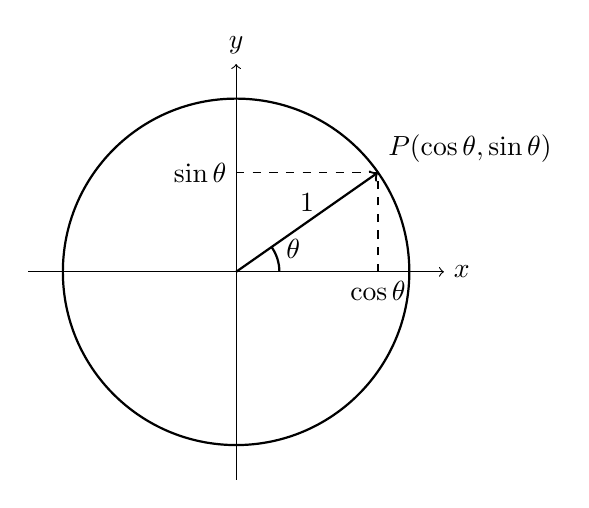
\begin{tikzpicture}[scale=2.2]
    % Unit circle
    \draw[thick] (0,0) circle (1);
    % Axes
    \draw[->] (-1.2,0) -- (1.2,0) node[right] {$x$};
    \draw[->] (0,-1.2) -- (0,1.2) node[above] {$y$};
    % Radius
    \draw[->, thick] (0,0) -- ({cos(35)},{sin(35)}) 
        node[midway,above] {$1$}
        node[above right] {$P(\cos\theta,\sin\theta)$};
    % Projection lines
    \draw[dashed] ({cos(35)},0) -- ({cos(35)},{sin(35)});
    \draw[dashed] (0,{sin(35)}) -- ({cos(35)},{sin(35)});
    % Labels
    \node[below] at ({cos(35)},0) {$\cos\theta$};
    \node[left]  at (0,{sin(35)}) {$\sin\theta$};
    % Angle arc
    \draw[thick] (0.25,0) arc (0:35:0.25);
    \node at (0.33,0.13) {$\theta$};
\end{tikzpicture}
\caption{The unit circle, $x^{2}+y^{2}=1$, showing the geometric meaning of $\sin\theta$ and $\cos\theta$.}
\end{figure}

\subsection{Parametric Form of Trigonometric Functions}

In mathematics, parametric equations describe a curve by expressing its
coordinates as functions of a single independent variable called a
\textbf{parameter}.

The familiar \textbf{geometrical definitions} based on a right-angled triangle,
\[
\cos\theta = \frac{\text{adjacent}}{\text{hypotenuse}}, \qquad
\sin\theta = \frac{\text{opposite}}{\text{hypotenuse}}, \qquad
\tan\theta = \frac{\sin\theta}{\cos\theta},
\]
can be naturally re-expressed using coordinates on the \textbf{unit circle}
($r=1$).

If $\theta$ is the angle measured anticlockwise from the positive $x$-axis to
the radius $OP$, then the right-angled triangle formed by $O$, $P$, and the
projection of $P$ onto the $x$-axis has:
\[
\text{adjacent side} = x, \qquad
\text{opposite side} = y, \qquad
\text{hypotenuse} = 1.
\]

Hence, for the unit circle,
\[
\cos\theta = \frac{x}{1} = x, \qquad
\sin\theta = \frac{y}{1} = y.
\]

Taking the angle $\theta$ as the parameter gives the parametric form of the
circle:
\[
x(\theta)=\cos\theta,\qquad y(\theta)=\sin\theta \qquad (0\le\theta<2\pi),
\]
so every point $(\cos\theta,\sin\theta)$ lies on the curve $x^2+y^2=1$.

Thus, the trigonometric functions $\cos\theta$ and $\sin\theta$ provide a
complete parametric description of the unit circle, with $\theta$ acting as the
parameter.

From this geometric viewpoint, many familiar properties of the trigonometric
functions follow naturally. The identity $\sin^2\theta+\cos^2\theta=1$ comes
directly from the circle equation $x^2+y^2=1$, symmetry reflects the axial
symmetry of the circle, and periodicity arises because rotating a full $2\pi$
returns a point to its original position.

It is worth recalling these facts, because many of the structural features of
trigonometry — including identities, symmetry, and reciprocal relationships —
will reappear when we explore hyperbolic functions. Trigonometric functions also
provide important models for circular motion, oscillations, waves, and other
periodic behaviours in mathematics, physics, and engineering.

\subsection{Circular Functions to Hyperbolic Functions}
Just as trigonometric functions arise from points traversing the unit circle,
hyperbolic functions have their geometric origin in the rectangular (or
equilateral) unit hyperbola, which is why they are called \emph{hyperbolic}
functions.
The rectangular unit hyperbola has the standard equation
\[
x^2 - y^2 = 1,
\]
with asymptotes along the lines $y = \pm x$ (forming right angles, hence the
term ``rectangular'').
\begin{figure}[htbp]
\centering
\begin{tikzpicture}[scale=1.9]
    % Axes
    \draw[->] (-2.3,0) -- (2.3,0) node[right] {$x$};
    \draw[->] (0,-2.3) -- (0,2.3) node[above] {$y$};
    % Hyperbola branches x^2 - y^2 = 1
    \draw[thick, domain=1:2.2, samples=200]
        plot (\x, {sqrt(\x*\x -1)});
    \draw[thick, domain=1:2.2, samples=200]
        plot (\x, {-sqrt(\x*\x -1)});
    \draw[thick, domain=-2.2:-1, samples=200]
        plot (\x, {sqrt(\x*\x -1)});
    \draw[thick, domain=-2.2:-1, samples=200]
        plot (\x, {-sqrt(\x*\x -1)});
    % Asymptotes y = x and y = -x
    \draw[dashed,gray] (-2.2,-2.2) -- (2.2,2.2);
    \draw[dashed,gray] (-2.2,2.2) -- (2.2,-2.2);
    \node[gray] at (1.7,1.55) {$y=x$};
    \node[gray] at (1.7,-1.55) {$y=-x$};
    % Choose t = 0.8
    \pgfmathsetmacro{\t}{0.8}
    \pgfmathsetmacro{\X}{cosh(\t)}
    \pgfmathsetmacro{\Y}{sinh(\t)}
    % Point on hyperbola
    \filldraw[blue] (\X,\Y) circle (1.5pt)
      node[right] {$\,(\cosh t,\ \sinh t)$};
    % Projection lines
    \draw[dashed] (\X,0) -- (\X,\Y);
    \draw[dashed] (0,\Y) -- (\X,\Y);
    % Labels
    \node[below] at (\X,0) {$\cosh t$};
    \node[left] at (0,\Y) {$\sinh t$};
\end{tikzpicture}
\caption{The rectangular hyperbola $x^2 - y^2 = 1$ with a point parameterised by $(\cosh t,\sinh t)$.}
\end{figure}

Points on its right-hand branch ($x \ge 1$) can be parameterised as
\[
(\cosh t,\ \sinh t) \qquad (t \in \mathbb{R}),
\]
mirroring how points on the unit circle
\[
x^2 + y^2 = 1
\]
are described by
\[
(\cos\theta,\ \sin\theta) \qquad (\theta \in [0,2\pi)).
\]
Here, the letter ``h'' indicates that these are \emph{hyperbolic} versions of the
familiar cosine and sine.
The parallel between the two settings (circular functions and hyperbolic functions) is also seen in their fundamental identities:
\begin{itemize}
    \item \textbf{Unit Circle} ($x^2 + y^2 = 1$) The fundamental identity is:
    \begin{equation*}
        \cos^2\theta + \sin^2\theta = 1
    \end{equation*}
    \item \textbf{Unit Hyperbola} ($x^2 - y^2 = 1$) The fundamental identity is:
    \begin{equation*}
        \cosh^2 t - \sinh^2 t = 1
    \end{equation*}
\end{itemize}

\subsection{Parametric Form of Trigonometric Functions}

In mathematics, parametric equations describe a curve by expressing its
coordinates as functions of a single independent variable called a
\textbf{parameter}.

The familiar \textbf{geometrical definitions} based on a right-angled triangle,
\[
\cos\theta = \frac{\text{adjacent}}{\text{hypotenuse}}, \qquad
\sin\theta = \frac{\text{opposite}}{\text{hypotenuse}}, \qquad
\tan\theta = \frac{\sin\theta}{\cos\theta},
\]
can be naturally re-expressed using coordinates on the \textbf{unit circle}
($r=1$).

If $\theta$ is the angle measured anticlockwise from the positive $x$-axis to
the radius $OP$, then the right-angled triangle formed by $O$, $P$, and the
projection of $P$ onto the $x$-axis has:
\[
\text{adjacent side} = x, \qquad
\text{opposite side} = y, \qquad
\text{hypotenuse} = 1.
\]

Hence, for the unit circle,
\[
\cos\theta = \frac{x}{1} = x, \qquad
\sin\theta = \frac{y}{1} = y.
\]

Taking the angle $\theta$ as the parameter gives the parametric form of the
circle:
\[
x(\theta)=\cos\theta,\qquad y(\theta)=\sin\theta \qquad (0\le\theta<2\pi),
\]
so every point $(\cos\theta,\sin\theta)$ lies on the curve $x^2+y^2=1$.

Thus, the trigonometric functions $\cos\theta$ and $\sin\theta$ provide a
complete parametric description of the unit circle, with $\theta$ acting as the
parameter.

From this geometric viewpoint, many familiar properties of the trigonometric
functions follow naturally. The identity $\sin^2\theta+\cos^2\theta=1$ comes
directly from the circle equation $x^2+y^2=1$, symmetry reflects the axial
symmetry of the circle, and periodicity arises because rotating a full $2\pi$
returns a point to its original position.

It is worth recalling these facts, because many of the structural features of
trigonometry — including identities, symmetry, and reciprocal relationships —
will reappear when we explore hyperbolic functions. Trigonometric functions also
provide important models for circular motion, oscillations, waves, and other
periodic behaviours in mathematics, physics, and engineering.

\subsection{Circular Functions to Hyperbolic Functions}
Just as trigonometric functions arise from points traversing the unit circle,
hyperbolic functions have their geometric origin in the rectangular (or
equilateral) unit hyperbola, which is why they are called \emph{hyperbolic}
functions.
The rectangular unit hyperbola has the standard equation
\[
x^2 - y^2 = 1,
\]
with asymptotes along the lines $y = \pm x$ (forming right angles, hence the
term ``rectangular'').
\begin{figure}[htbp]
\centering
\begin{tikzpicture}[scale=1.9]
    % Axes
    \draw[->] (-2.3,0) -- (2.3,0) node[right] {$x$};
    \draw[->] (0,-2.3) -- (0,2.3) node[above] {$y$};
    % Hyperbola branches x^2 - y^2 = 1
    \draw[thick, domain=1:2.2, samples=200]
        plot (\x, {sqrt(\x*\x -1)});
    \draw[thick, domain=1:2.2, samples=200]
        plot (\x, {-sqrt(\x*\x -1)});
    \draw[thick, domain=-2.2:-1, samples=200]
        plot (\x, {sqrt(\x*\x -1)});
    \draw[thick, domain=-2.2:-1, samples=200]
        plot (\x, {-sqrt(\x*\x -1)});
    % Asymptotes y = x and y = -x
    \draw[dashed,gray] (-2.2,-2.2) -- (2.2,2.2);
    \draw[dashed,gray] (-2.2,2.2) -- (2.2,-2.2);
    \node[gray] at (1.7,1.55) {$y=x$};
    \node[gray] at (1.7,-1.55) {$y=-x$};
    % Choose t = 0.8
    \pgfmathsetmacro{\t}{0.8}
    \pgfmathsetmacro{\X}{cosh(\t)}
    \pgfmathsetmacro{\Y}{sinh(\t)}
    % Point on hyperbola
    \filldraw[blue] (\X,\Y) circle (1.5pt)
      node[right] {$\,(\cosh t,\ \sinh t)$};
    % Projection lines
    \draw[dashed] (\X,0) -- (\X,\Y);
    \draw[dashed] (0,\Y) -- (\X,\Y);
    % Labels
    \node[below] at (\X,0) {$\cosh t$};
    \node[left] at (0,\Y) {$\sinh t$};
\end{tikzpicture}
\caption{The rectangular hyperbola $x^2 - y^2 = 1$ with a point parameterised by $(\cosh t,\sinh t)$.}
\end{figure}

Points on its right-hand branch ($x \ge 1$) can be parameterised as
\[
(\cosh t,\ \sinh t) \qquad (t \in \mathbb{R}),
\]
mirroring how points on the unit circle
\[
x^2 + y^2 = 1
\]
are described by
\[
(\cos\theta,\ \sin\theta) \qquad (\theta \in [0,2\pi)).
\]
Here, the letter ``h'' indicates that these are \emph{hyperbolic} versions of the
familiar cosine and sine.
The parallel between the two settings (circular functions and hyperbolic functions) is also seen in their fundamental identities:
\begin{itemize}
    \item \textbf{Unit Circle} ($x^2 + y^2 = 1$) The fundamental identity is:
    \begin{equation*}
        \cos^2\theta + \sin^2\theta = 1
    \end{equation*}
    \item \textbf{Unit Hyperbola} ($x^2 - y^2 = 1$) The fundamental identity is:
    \begin{equation*}
        \cosh^2 t - \sinh^2 t = 1
    \end{equation*}
\end{itemize}

\subsection{Parametric Form of Hyperbolic Functions}

Just as points on the unit circle can be written in parametric form as
\[
x = \cos\theta, \qquad y = \sin\theta \qquad (\theta \in [0,2\pi)),
\]
points on the right-hand branch of the rectangular unit hyperbola
\[
x^2 - y^2 = 1
\]
can be expressed in the parametric form
\[
x = \cosh t, \qquad y = \sinh t \qquad (t \in \mathbb{R}).
\]

The corresponding hyperbolic functions are defined using the exponential forms
\[
\sinh t = \frac{e^t - e^{-t}}{2}, \qquad
\cosh t = \frac{e^t + e^{-t}}{2}, \qquad
\tanh t = \frac{\sinh t}{\cosh t}.
\]

These expressions are not chosen arbitrarily: substituting them into the
hyperbola equation shows precisely why they parametrise it:
\[
\cosh^2 t - \sinh^2 t = 1.
\]

\begin{align*}
\cosh^2 t - \sinh^2 t
&= \left( \frac{e^t + e^{-t}}{2} \right)^2
   - \left( \frac{e^t - e^{-t}}{2} \right)^2 \\
&= \frac{(e^t + e^{-t})^2 - (e^t - e^{-t})^2}{4} \\
&= \frac{ [e^{2t} + 2 + e^{-2t}] - [e^{2t} - 2 + e^{-2t}] }{4} \\
&= \frac{4}{4} = 1.
\end{align*}

Thus, every point $(\cosh t,\sinh t)$ lies on the hyperbola $x^2-y^2=1$, tracing
its right branch as $t$ varies through all real numbers (with $\cosh t \ge 1$
and $\sinh t$ ranging over all real values).

Geometrically, $\cosh t$ gives the $x$-coordinate (always $\ge 1$) and $\sinh t$ the $y$-coordinate, playing roles analogous to $\cos\theta$ and $\sin\theta$ on the unit circle. However, unlike circular trigonometry, which is inherently periodic, hyperbolic functions are based on exponentials, so they exhibit smooth, unbounded growth.

Hyperbolic functions frequently arise in contexts involving balanced forces,
equilibrium shapes, and growth curves. A classical example is the
\textbf{catenary}, the curve formed by a hanging chain, which is a scaled
version of $\cosh x$.

\subsection{Comparing Trigonometric and Hyperbolic Properties}

Although trigonometric and hyperbolic functions arise from different geometric
curves (the unit circle and the rectangular unit hyperbola), they share many
structural similarities. The table below highlights some key parallels and
contrasts between the two families.

\begin{table}[h!]
\centering
\renewcommand{\arraystretch}{1.4}
\begin{tabular}{|l|p{5cm}|p{5cm}|}
\hline
\textbf{Property} &
\textbf{Trigonometric Functions} &
\textbf{Hyperbolic Functions} \\ \hline

\textbf{Symmetry} &
$\sin(-x) = -\sin x$ \ (odd) \newline
$\cos(-x) = \cos x$  \ (even) \newline
$\tan(-x) = -\tan x$ \ (odd) &
$\sinh(-x) = -\sinh x$ \ (odd) \newline
$\cosh(-x) = \cosh x$  \ (even) \newline
$\tanh(-x) = -\tanh x$ \ (odd) \\ \hline

\textbf{Fundamental Identity} &
$\sin^2 x + \cos^2 x = 1$ &
$\cosh^2 x - \sinh^2 x = 1$
\newline (note the reversed sign) \\ \hline

\textbf{Behaviour and Range} &
$\sin x,\cos x$ oscillate between $-1$ and $1$ \newline
(periodic behaviour) \newline
$-1 < \tan x < 1$ only on restricted intervals &
$\cosh x \ge 1$ for all real $x$ \newline
$-1 < \tanh x < 1$ for all real $x$ \newline
$\tanh x \to \pm 1$ as $x \to \pm\infty$ \newline
(non-periodic behaviour) \\ \hline

\textbf{Graphs} &
Wave-like, repeating patterns \newline
(periodic with amplitude bounded by $\pm1$) &
Smooth, non-periodic curves \newline
(reflecting exponential growth and decay) \\ \hline

\end{tabular}
\caption{Comparison of key properties of circular (trigonometric) and hyperbolic functions.}
\end{table}

\subsection{Reciprocal Hyperbolic Functions}

As in ordinary trigonometry, we also define the reciprocal functions:
\[
\cosech x = \frac{1}{\sinh x}, \qquad
\sech x   = \frac{1}{\cosh x}, \qquad
\coth x   = \frac{1}{\tanh x}.
\]

\begin{itemize}
    \item $\cosech x$ and $\coth x$ are undefined at $x=0$,
    because $\sinh 0 = 0$ and $\tanh 0 = 0$.
    \item $\sech x$ is defined for all real $x$ because $\cosh x$ never becomes
    zero.
\end{itemize}

\subsection{Why Study Hyperbolic Functions?}

Hyperbolic functions have:
\begin{itemize}
    \item inverse forms that can be written using logarithms,
    \item a wide range of identities,
    \item important uses in integration,
    \item and applications in real-world modelling, such as catenary arches,
    suspension bridges and power cable curves.
\end{itemize}

They form an important part of Further Pure Mathematics, linking exponential
expressions with geometry, calculus and physical modelling.

\clearpage
\section{Questions}

\subsection{Edexcel IAL FP3}

\noindent\textbf{Q1 -- January 2022} 
\begin{enumerate}
    \item[(a)] Use the definitions of hyperbolic functions in terms of exponentials to prove that
    \[
        8\cosh^4 x = \cosh 4x + p\,\cosh 2x + q
    \]
    where $p$ and $q$ are constants to be determined.
    \hfill (3)

    \item[(b)] Hence, or otherwise, solve the equation
    \[
        \cosh 4x - 17\cosh 2x + 9 = 0
    \]
    giving your answers in exact simplified form in terms of natural logarithms.
    \hfill (5)
\end{enumerate}

\noindent\textbf{Solution:}
\begin{enumerate}
    \item[(a)] \textbf{Using exponentials to find $p$ and $q$.}

    From the definition
    \[
        \cosh x = \frac{e^x + e^{-x}}{2},
    \]
    we have
    \[
        \cosh^2 x
        = \left(\frac{e^x + e^{-x}}{2}\right)^2
        = \frac{e^{2x} + 2 + e^{-2x}}{4}
        = \frac{1}{2}\bigl(\cosh 2x + 1\bigr).
    \]
    Hence
    \[
        \cosh^4 x
        = \left(\cosh^2 x\right)^2
        = \left(\frac{\cosh 2x + 1}{2}\right)^2
        = \frac{1}{4}\Big(\cosh^2 2x + 2\cosh 2x + 1\Big).
    \]
    Using again
    \[
        \cosh^2 2x = \frac{1}{2}\bigl(\cosh 4x + 1\bigr),
    \]
    we obtain
    \[
        8\cosh^4 x
        = 2\cosh^2 2x + 4\cosh 2x + 2
        = 2\cdot\frac{\cosh 4x + 1}{2} + 4\cosh 2x + 2.
    \]
    Therefore
    \[
        8\cosh^4 x
        = \cosh 4x + 1 + 4\cosh 2x + 2
        = \cosh 4x + 4\cosh 2x + 3.
    \]
    Comparing with
    \[
        8\cosh^4 x = \cosh 4x + p\cosh 2x + q,
    \]
    we find
    \[
        p = 4, \qquad q = 3.
    \]

    \item[(b)] \textbf{Solving $\cosh 4x - 17\cosh 2x + 9 = 0$.}

    Using the identity
    \[
        \cosh 4x = 2\cosh^2 2x - 1,
    \]
    the given equation becomes
    \[
        2\cosh^2 2x - 1 - 17\cosh 2x + 9 = 0,
    \]
    that is
    \[
        2\cosh^2 2x - 17\cosh 2x + 8 = 0.
    \]
    Let
    \[
        y = \cosh 2x.
    \]
    Then
    \[
        2y^2 - 17y + 8 = 0.
    \]
    Solving,
    \[
        (y - 8)(2y - 1) = 0,
    \]
    so
    \[
        y = 8 \quad \text{or} \quad y = \frac{1}{2}.
    \]

    Since $\cosh 2x \ge 1$ for all real $x$, $y=\tfrac12$ is impossible. Thus
    \[
        \cosh 2x = 8.
    \]
    Using the inverse hyperbolic cosine,
    \[
        2x = \cosh^{-1}(8)
        = \ln\!\left(8 + \sqrt{8^2 - 1}\,\right)
        = \ln\!\left(8 + \sqrt{63}\right),
    \]
    where
    \[
        \cosh^{-1}a = \ln(a + \sqrt{a^2 - 1}), \qquad a \ge 1.
    \]

    As $\cosh$ is even, both signs are possible:
    \[
        2x = \pm\,\cosh^{-1}(8).
    \]
    Hence
    \[
        x = \pm\,\frac{1}{2}\cosh^{-1}(8)
          = \pm\,\frac{1}{2}\ln\!\left(8 + \sqrt{63}\right).
    \]

    \medskip

    \noindent\textbf{Final answer:}
    \[
        x = \pm\frac{1}{2}\ln\!\left(8 + \sqrt{63}\right).
    \]
\end{enumerate}

\noindent\textbf{Q1 -- June 2009 }

Solve the equation $ \operatorname{sech}x \;-\; \tanh x \;=\; 5 $

\noindent\textbf{Solution:}

Using the exponential definitions
\[
\operatorname{sech}x = \frac{2}{e^x + e^{-x}}, 
\qquad
\tanh x = \frac{e^x - e^{-x}}{\,e^x + e^{-x}\,},
\]
let \( t = e^x \) (so \(t>0\)), which gives \( e^{-x} = \tfrac{1}{t} \). Then
\[
\operatorname{sech}x = \frac{2}{t+\tfrac{1}{t}}
= \frac{2t}{t^2+1},
\qquad
\tanh x = \frac{t - \tfrac{1}{t}}{t + \tfrac{1}{t}}
= \frac{t^2 - 1}{t^2+1}.
\]

Substituting into the equation:
\[
\frac{2t}{t^2+1}
\;-\;
\frac{t^2-1}{t^2+1}
\;=\;
5.
\]

Multiply through by \(t^2+1\):
\[
2t - (t^2 - 1) = 5(t^2 + 1).
\]

Expand and simplify:
\[
2t - t^2 + 1 = 5t^2 + 5,
\]
\[
0 = 6t^2 - 2t + 4,
\]
\[
3t^2 - t + 2 = 0.
\]

Factorising:
\[
(3t - \dots)(t - \dots) = 0. \quad \text{(Note: The correct factorization gives only one real solution for } x.)
\]

\noindent\textbf{Q3 -- Jun 2010}
\begin{enumerate}
    \item[(a)] Starting from the definitions of $\sinh x$ and $\cosh x$ in terms
    of exponentials, prove that
    \[
        \cosh 2x = 1 + 2\sinh^2 x.
    \]
    \hfill (3)

    \item[(b)] Solve the equation
    \[
        \cosh 2x - 3\sinh x = 15,
    \]
    giving your answers as exact logarithms.
    \hfill (5)
\end{enumerate}


\noindent\textbf{Q5 -- June 2011}

The curve $C_1$ has equation $y = 3\sinh 2x$, and the curve $C_2$ has equation $y = 13 - 3e^{2x}$.
\begin{enumerate}
    \item[(a)] Sketch the graph of the curves $C_1$ and $C_2$ on one set of axes,
    giving the equation of any asymptote and the coordinates of points where the
    curves cross the axes.
    \hfill (4)

    \item[(b)] Solve the equation
    \[
        3\sinh 2x = 13 - 3e^{2x},
    \]
    giving your answer in the form $\dfrac{1}{2}\ln k$, where $k$ is an integer.
    \hfill (5)
\end{enumerate}

\noindent\textbf{Q7 - June 2012} 

Let $ f(x) = 5\cosh x - 4\sinh x, \qquad x \in \mathbb{R}$.
\begin{enumerate}
    \item[(a)] Show that
    \[
        f(x) = \frac{1}{2}\bigl(e^x + 9e^{-x}\bigr).
    \]
    \hfill (2)

    \item[(b)] Hence solve the equation
    \[
        f(x) = 5.
    \]
    \hfill (4)

    \item[(c)] Hence show that
    \[
        \int_{\tfrac{1}{2}\ln 3}^{\ln 3} \frac{1}{5\cosh x - 4\sinh x}\,dx
        = \frac{\pi}{18}.
    \]
    \hfill (5)
\end{enumerate}


\end{document}